\documentclass[11pt]{article}
\usepackage{personal_commands}
\usepackage[italian]{babel}

\title{\textbf{Note del corso di Analisi Matematica 1}}
\author{Gabriel Antonio Videtta}
\date{17 marzo 2023}

\begin{document}

\maketitle

\begin{center}
    \Large \textbf{Successioni per ricorrenza}
\end{center}

\begin{remark}
Sia $X$ l'insieme delle successioni a valori reali che soddisfano una data
eq.~ricorsiva lineare ed omogenea di ordine $k$ (ossia che coinvolge
$k$ precedenti elementi di una successione). \\

\li $X$ è uno spazio vettoriale su $\RR$. \\
\li $T : X \to \RR^n$, $(x_n) \mapsto (x_0, ..., x_{k-1})^\top$ è
un isomorfismo, e quindi $\dim X = k$. \\
\li Si può facilmente individuare una base naturale di $X$, costituita dagli
elementi della forma $\vec{x_i} = T\inv(\vec{e_ {i + 1}})$ con $i = 0, ..., k - 1$,
dove $\vec{x_i}$ rappresenta una successione di $X$ dove l'$i$-esimo elemento
è pari a $1$ e gli altri, tra $0$ e $k-1$, sono nulli.
\end{remark}

\begin{remark}
Le eq.~differenziali ordinarie si possono approssimare
ad eq.~su differenze finite (e questa considerazione è
alla base della grande somiglianza tra i concetti sviluppati
sia per queste che per quelle).
\end{remark}

\begin{example} (ricondursi a un caso discreto) 
Si consideri un'eq.~differenziale omogenea lineare del primo
ordine su $x(t)$. Si può approssimare $t$ con $nh$, dato
$h$ piccolo, e così scrivere $x_n = x(nh) \approx x(t)$.
Così, allora, $x_{n+1} = x((n+1)h) = x(t + h)$. Conseguentemente $h
x'(t) \approx x(t + h) - x(t) \approx x_{n+1} - x_n$. \\

Si provi a risolvere, per esempio, l'eq.~ differenziale $x'(t) = x(t)$.
Sostituendo, si ottiene $x_{n+1} - x_n = h x_n$, da cui
si ricava l'eq.~ricorsiva $x_{n+1} = (1 + h) x_n$. Allora
$x(nh) = x_n = (1 + h)^n \underbrace{x(0)}_c = (1 + h)^n c$. \\

In effetti $x(t) = \displaystyle \lim_{h \to 0} (1 + h)^n c =
\lim_{h \to 0} \left[(1 + h)^{\frac{1}{h}}\right]^t c = c e^t$,
la famiglia di soluzioni dell'eq.~differenziale originale.
\end{example}

\begin{example} (metodo delle bisettrici)
Sia data la sequente successione:

\[ (x_n) = \begin{cases} x_n = x_{n-1}^4, \\ x_0 = \frac12. \end{cases} \]

Si consideri allora il sistema di funzioni:

\[ \begin{cases}
    f(x) = x^4, \\ y = x,
\end{cases} \]

ossia i punti fissi di $f(x)$. Si può disegnare facilmente
la successione mediante il seguente algoritmo: si prenda
$x_0$ sull'asse delle ascisse, e si valuti $f(x_0) = x_1$ collegando
il punto $(x_0, 0)$ a $(x_0, x_1)$,
alla fine ricollegato sulla bisettrice al punto $(x_1, x_1)$;
si colleghi $(x_1, x_1)$ a $(x_1, x_2 = f(x_1))$ e quest'ultimo a
$(x_2, x_2)$, etc. Si sarà allora
disegnato in modo grafico la successione, e considerando
i blocchi che connettono $(x_{n-1}, x_{n-1})$, $(x_{n-1}, x_n)$
e $(x_n, x_n)$, si potrà facilmente intuire che $x_n \tendston \infty$ per $x_0 > 1$, che $x_n \tendston 1$ per $x_0 = 1$,
e che $x_n \tendston 0$ per $x_0 < 1$. Quindi nel caso
dell'esempio, $x_n \tendston 0$.

\begin{figure}[H]
    \centering
    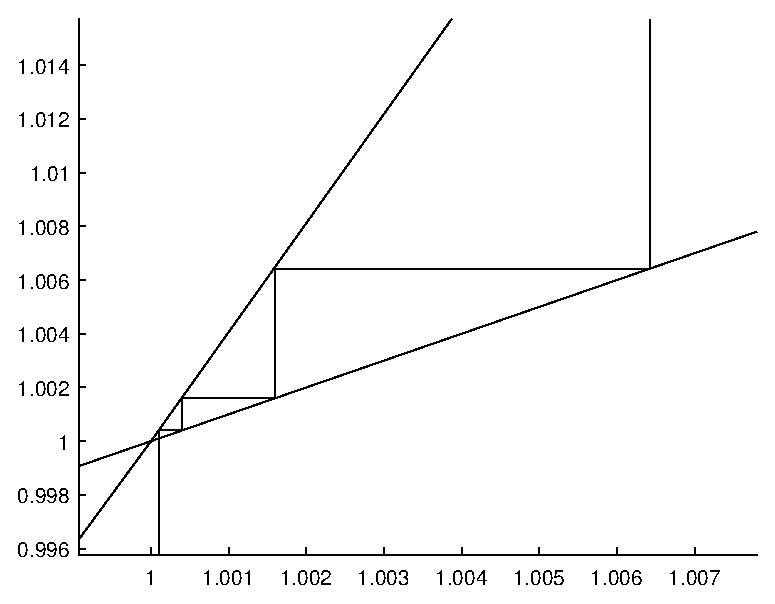
\includegraphics[width=0.6\textwidth]{esempio.eps}
    \caption{Applicazione dell'algoritmo con $x_0 = 1,0001$.}
    \label{fig:my_label}
\end{figure}

\end{example}

\begin{example}
    Riprendendo l'esempio precedente, si può ora provare
    a dimostrare formalmente i risultati ottenuti.
    Sempre graficamente, si intuisce che $(x_n)$ sarà
    decrescente, e quindi che ammetterà limite (che,
    in particolare, coinciderà con il suo estremo inferiore). \\

    Si dimostra quindi, per prima cosa, che $(x_n)$ è
    decrescente, e che vale $0 \leq x_n \leq \frac{1}{2}$.
    Si procede per induzione: se $n=0$, la tesi è già
    verificata; se la tesi è vera fino a $n-1$, allora
    $x_n = \underbrace{x_{n-1}^4}_{\geq 0} \leq \left(\frac{1}{2}\right)^4 = \frac{1}{16} \leq \frac{1}{2}$. Quindi
    $(x_n)$ è decrescente, e poiché $0$ ne è minorante,
    varrà in particolare che $\ell = \lim_{n \to \infty} x_n \in [0, \frac{1}{2}]$. \\

    Si mostra che $\ell$ deve essere un punto fisso di
    $f$: poiché $x_n \tendston \ell$, anche $x_{n+1} \tendston
    \ell$ (essendone una sottosuccessione); inoltre, poiché
    $x_{n+1} = x_n^4$, $x_{n+1} \tendston \ell^4$. Poiché il limite è unico, deve allora valere $\ell = \ell^4 = f(\ell)$. Poiché gli unici punti di fissi di $f$ sono
    $0$ e $1$, e $1$ non è
    minorante di $(x_n)$,
    deve valere che $\ell = 0$. \\

    Se invece $x_0$ fosse stato
    maggiore di $1$, si sarebbe
    dimostrato che $(x_n)$ era
    strettamente crescente, e
    dunque avrebbe ammesso comunque
    limite; tale limite non sarebbe
    potuto essere né $0$ né $1$,
    dacché non sarebbero stati maggioranti
    di $(x_n)$, né tantomeno
    $-\infty$. Allora tale limite
    avrebbe dovuto essere,
    forzatamente, $\infty$.
\end{example}

\begin{example}
    Si consideri adesso la
    successione:

    \[ \begin{cases}
        x_0 = 2, \\
        x_{n+1} = \frac{x_n}{2} + \frac{1}{x_n}.
    \end{cases} \]

    Applicando lo stesso ragionamento
    di prima, si considera $f(x) = \frac{x}{2} + \frac{2}{x}$. È sufficiente
    dimostrare che $(x_n)$ è tale che
    $\sqrt{2} \leq x_n \leq 2$
    $\forall n \in \NN$ (dove $\sqrt{2}$
    è l'unico punto fisso di $f(x)$) per
    concludere immediatamente che
    il limite di tale successione è
    proprio $\sqrt{2}$.
\end{example}

\begin{example}
    Si consideri l'eq.~ricorsiva $x_n = \frac{1}{x_{n-1}^2}$,
    con $x_0 > 1$.
    Qualsiasi disegno si faccia, si osserverà una "spirale"
    nella configurazione della successione: si ipotizzerà
    dunque che $x_n$ non ammetterà limite. Si distinguono
    dal disegno due sottosuccessioni: $x_{2n}$ e $x_{2n+1}$,
    che, rispettivamente, obbediranno a due eq.~ricorsive,
    $x_{2(n+1)} = x_{2n}^4$ e $x_{2(n+1) + 1} = x_{2n + 1}^4$,
    ossia la successione analizzata in uno scorso esempio. \\

    \begin{figure}[H]
        \centering
        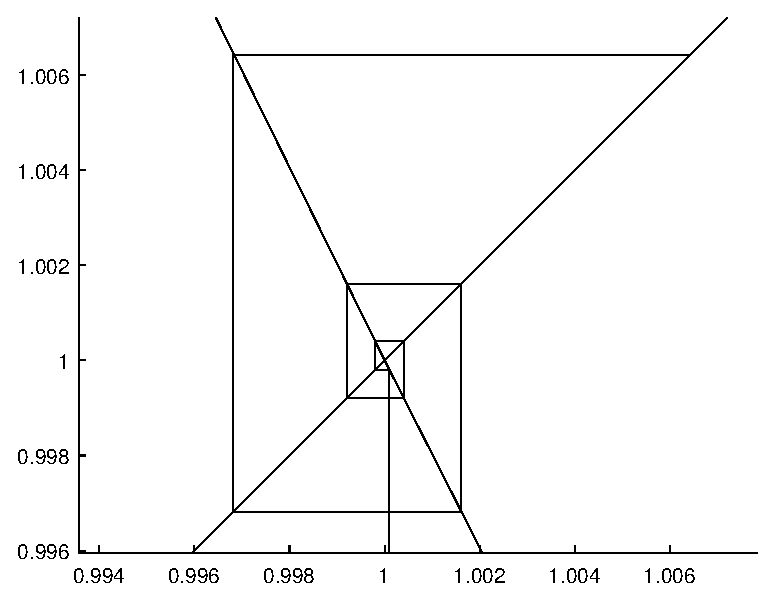
\includegraphics[width=0.6\textwidth]{esempio2.eps}
        \caption{Applicazione del metodo della bisettrice con $x_0 = 1,0001$.}
        \label{fig:my_label}
    \end{figure}

    Poiché $x_0 > 1$, $x_1 = \frac{1}{x_0^2} < 1$. Allora
    $x_{2n} \tendston \infty$, mentre $x_{2n+1} \tendston
    0$: poiché una sottosuccessione deve tendere allo
    stesso limite della successione da cui deriva, ed il
    limite è unico, si conclude che $(x_n)$ non ammette
    limite.
\end{example}

\end{document}
